% Appendix D: Calibration against analytic limits and reference models
%
% Structure: eight named calibrations in the BHL/Hamilcar register,
% with the FV <-> TorsionCDT cross-formulation check as the central
% methodology for the complex PGT theories surveyed in §4. Every
% quantitative number traces to a benchmark in scripts/benchmarks/,
% a canonical JSON in benchmark_results/canonical/, and a figure
% script in scripts/figures/ (publication manifest registers each
% round trip). Headline corpus tics: avoid `pipeline`/`validate`;
% prefer `calibrate`/`reproduce`/`recover`/`agreement`/`sanity-check`/
% `audit`/`diagnostic`/`precision floor`.
%
% No internal git/issue/commit/date references appear in the prose;
% bugs surfaced by the calibration suite are described by what they
% were (with citations to the relevant numerical-methods literature),
% not by their tracker IDs. Example-library entries are referred to
% by their physics, not by their repository filenames.

\section{Calibration against analytic limits and reference models}%
\label{Validation}

\paragraph*{Boccaletti reproduction on a uniform background}
The Gertsenshtein conversion kernel of \cref{GertsenshteinFormula}
provides the closed-form analytic baseline against which we calibrate
\TIDAL{} on a uniform background magnetic field. We sweep $\Bzero$
over the perturbative regime with fourth-order finite-difference
operators on a periodic grid, and overlay the calibration data on
two analytic predictions: \cref{GertsenshteinFormula} and the Raffelt--Stodolsky two-mode formula with graviton-effective-mass
detuning~\cite{raffelt1988mixing},
\begin{equation}
  \begin{split}
    \Pconv &= \frac{g^2}{g^2 + \Delta^2}\,
      \sin^2\!\left(\sqrt{g^2+\Delta^2}\,D\right), \\
    g &= \frac{\kappa\Bzero}{2},
    \qquad \Delta = -\frac{\kappa^2 \Bzero^2}{4\omega},
  \end{split}
  \label{TwoModeRabi}
\end{equation}
in which $\omega \simeq k$ is the carrier angular frequency of the
photon mode in the massless-dispersion limit, and both the amplitude
prefactor and the oscillation frequency receive corrections from the
effective mass; the regime of validity follows
\cref{PerturbativityHierarchy}. The two predictions coincide while
$\kappa\Bzero t/2 \ll \pi/2$; the swept $\Bzero$ range extends just
into the saturated regime where they begin to differ visibly.
\Cref{BoccalettiUniform} displays the calibration overlay and the
multi-backend convergence at one regime point: modal and \CVODE{}
reach the FD-4 spatial-discretisation plateau at every grid size,
while leapfrog Yoshida-2 and Yoshida-4 converge toward the same
plateau from above as the CFL-controlled time step shrinks with
$\Delta x$. The reproduction calibrates the uniform-background
sector; localised-profile reproduction is calibrated separately in
\cref{BoccalettiLocalised}.

\begin{figure*}[t]
  \centering
  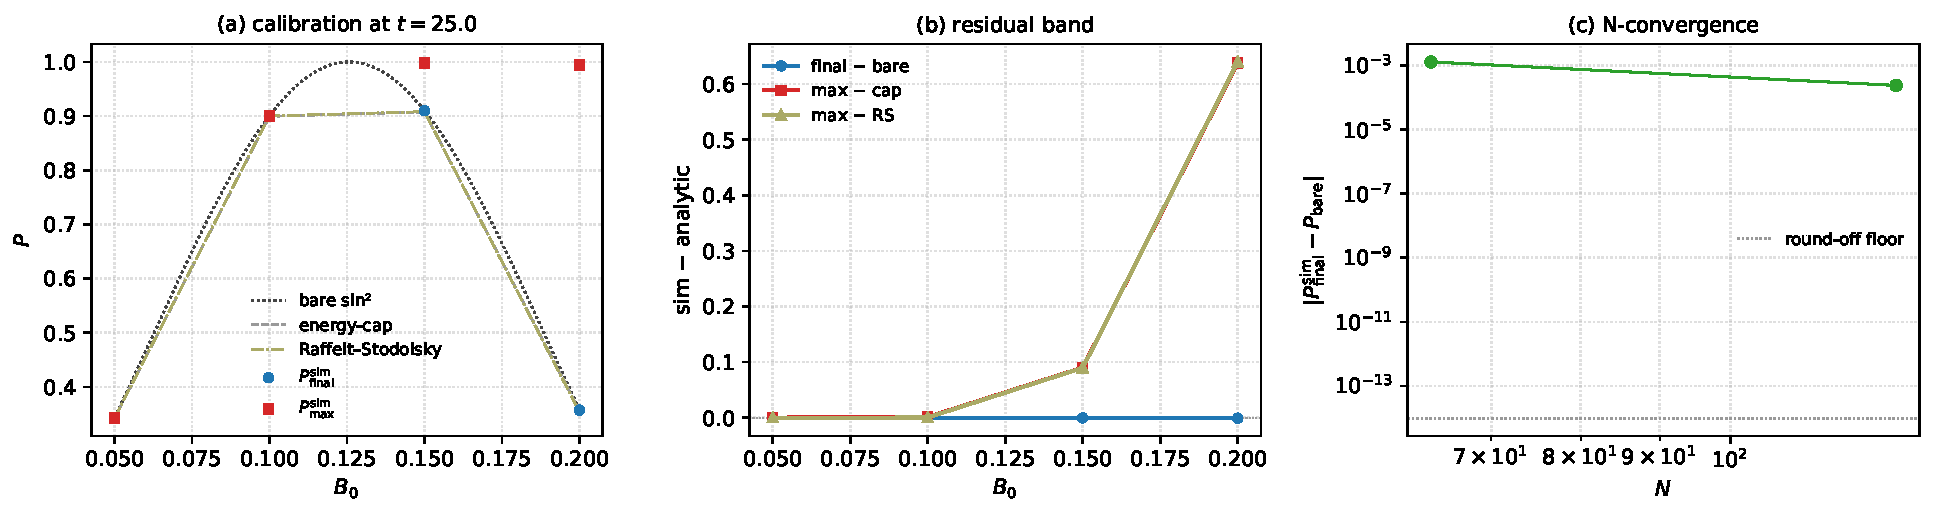
\includegraphics[width=\textwidth]{figures/figD_boccaletti_uniform}
  \caption{Boccaletti-kernel reproduction in the uniform-$\Bzero$
    regime. (a) Simulated $P_\mathrm{final}(\Bzero)$ at fixed
    $t_\mathrm{end}=50$ overlaid with the bare sin\textsuperscript{2}
    formula \cref{GertsenshteinFormula} and the Raffelt--Stodolsky two-mode
    formula \cref{TwoModeRabi}, the latter accounting for both the
    amplitude and frequency corrections from the graviton effective
    mass; the $\Bzero \in [0.005, 0.25]$ sweep is sampled at 24
    points on a periodic grid of $N=512$ points.
    (b) Convergence of
    $|P_\mathrm{final}^\mathrm{sim} - \sin^2(\kappa\Bzero t/2)|$ at
    the regime point $\Bzero = 0.1275$ on log--log axes for four
    solver backends (modal, \CVODE{}, leapfrog Yoshida-2, leapfrog
    Yoshida-4) at $N \in \{64, 128, 256, 512\}$. The
    tolerance-controlled backends (modal, \CVODE{}) reach the
    FD-4 spatial-discretisation plateau at every $N$; the
    symplectic backends converge toward the same plateau from above
    as the CFL-controlled time step shrinks with $\Delta x$.}
  \label{BoccalettiUniform}
\end{figure*}

\paragraph*{Path-integrated Boccaletti reproduction on a Gaussian profile}
For a finite magnetised region of profile $B_x(z)$ the Gertsenshtein
formula generalises to the path-integrated form
\begin{equation}
  \Pconv = \sin^2\!\left(
    \frac{\kappa}{2}\int_{-\infty}^{+\infty}\!B_x(z)\,\mathrm{d}z\right),
  \label{BoccalettiPathIntegrated}
\end{equation}
and for the Gaussian profile
$B_x(z) = B_\mathrm{peak}\exp(-z^2/(2R^2))$ the integral gives
$\Pconv = \sin^2(\kappa B_\mathrm{peak}\,R\sqrt{\pi/2})$. We
calibrate against this closed-form by sweeping the
$(B_\mathrm{peak}, R)$ plane using the derived localised
Gertsenshtein theory and a Gaussian wave-packet initial condition on
$h_+$ traversing the magnetised region. Neumann
boundary conditions are essential: the gauge potential
$\bar{A}_y \propto \mathrm{erf}(z/\sqrt{2}R)$ is non-periodic, and
periodic boundaries introduce spectral leakage that triggers spurious
exponential growth on tachyonic discrete modes (the failure mode
analysed in \cref{ICPreparation}). The strongest diagnostic is the
universal collapse of every cell onto the single curve
$P = \sin^2(s)$ in the dimensionless variable
$s = \kappa B_\mathrm{peak}\,R\sqrt{\pi/2}$. \Cref{BoccalettiLocalised}
displays the collapse. This calibrates the path-integrated kernel;
finite-frequency dispersion corrections are calibrated in
\cref{ConvergenceCalibration}.

\begin{figure}[t]
  \centering
  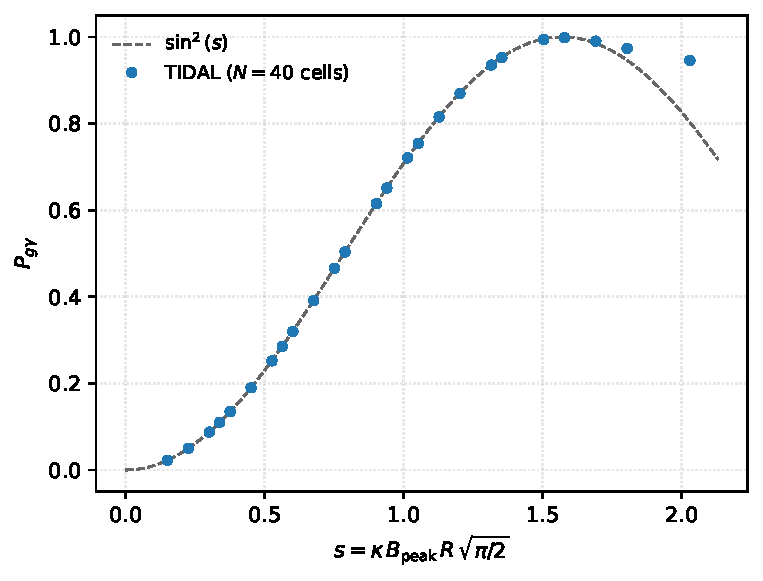
\includegraphics[width=\columnwidth]{figures/figD_boccaletti_localised}
  \caption{Path-integrated Boccaletti reproduction on the Gaussian
    profile. Universal collapse of every cell of an
    $8 \times 5$ $(B_\mathrm{peak}, R)$ grid onto the curve
    $P = \sin^2(s)$ in the dimensionless variable
    $s = \kappa B_\mathrm{peak}\,R\sqrt{\pi/2}$, on which the
    path-integrated prediction reduces to $\sin^2(s)$ regardless of
    the individual $(B_\mathrm{peak}, R)$ values. Points at
    $s > \pi/2$ (past the first quarter-period) lie below
    $\sin^{2}(s)$ as the bare-formula coherent approximation breaks
    down.}
  \label{BoccalettiLocalised}
\end{figure}

\paragraph*{Perturbed-Klein--Gordon calibration of the closed-form Duhamel kernel}
The perturbative-reduction machinery described in \cref{LPSReduction}
evolves the system as a base (order-$\varepsilon^{0}$) solution plus
a correction (order-$\varepsilon^{1}$), denoted \emph{Pass 0} and
\emph{Pass 1} in the figure legends below. We calibrate the kernel
against the analytical perturbative expansion of a Klein--Gordon
wave with a small mass-shift correction,
\begin{equation}
  \partial_t^2\phi - \partial_x^2\phi + m^2\phi
  \;=\; -\varepsilon\,\phi,
  \label{KGMassShift}
\end{equation}
whose full-$\varepsilon$ modal solution is closed-form. The
order-$\varepsilon^{0}$ solution evolves the $\varepsilon=0$ base;
the order-$\varepsilon^{1}$ correction is integrated against the
base trajectory; the combined approximation
$\phi^{(0)} + \phi^{(1)}$ matches the full solution to
$\mathcal{O}(\varepsilon^2)$ by construction. The log--log slope of
$|\phi^{(0)} + \phi^{(1)} - \phi^\mathrm{full}|$ versus $\varepsilon$
recovers the expected algebraic order, with an improvement ratio
over the base solution that grows as $1/\varepsilon$.
\Cref{ForcedOscillator} reports the error scaling and the fitted
slope.

\begin{figure}[t]
  \centering
  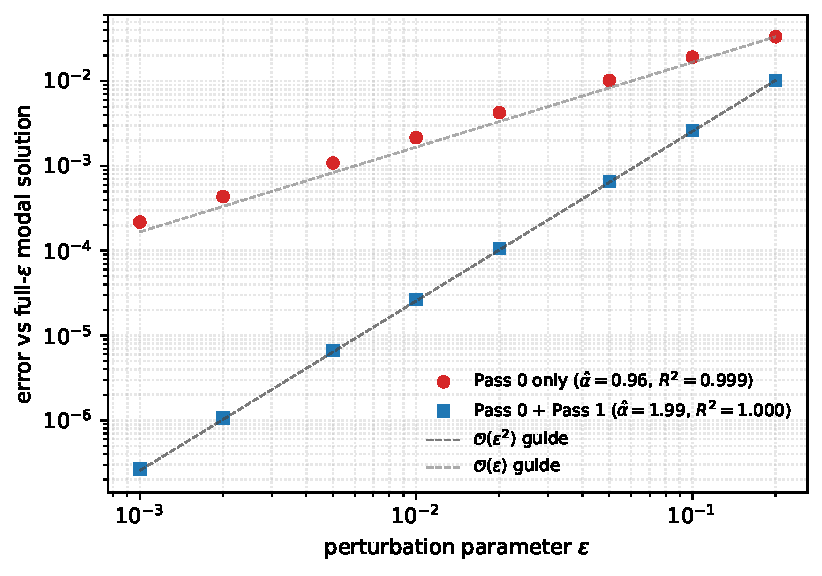
\includegraphics[width=\columnwidth]{figures/figD_forced_oscillator}
  \caption{Perturbed-Klein--Gordon calibration of the Pass 0 + Pass 1
    Duhamel kernel. Pass 0 error and combined Pass 0 + Pass 1 error
    versus $\varepsilon$ on log--log axes for the mass-shift correction
    \cref{KGMassShift}, sampled at eight logarithmically spaced
    points covering $\varepsilon \in [10^{-3}, 0.2]$ at $k=1$; fitted
    log--log slopes and $R^2$ values are reported in the legend. The
    Pass 0 + Pass 1 error scales as $\mathcal{O}(\varepsilon^2)$, an
    order of magnitude per half-decade in $\varepsilon$.}
  \label{ForcedOscillator}
\end{figure}

\paragraph*{Higher-derivative perturbative calibration}
We exercise the same order-$\varepsilon^{0,1}$ machinery on a
perturbative correction of distinct structure --- a fourth-order
spatial operator in place of the mass shift,
\begin{equation}
  \partial_t^2 \phi - \partial_x^2 \phi + m^2 \phi
  \;=\; -\varepsilon\,\partial_x^4 \phi,
  \label{KGBiharmonic}
\end{equation}
the canonical higher-derivative form encountered in the perturbative
reductions of \cite{parker1993reduced}. The base is the same
Klein--Gordon wave of \cref{KGMassShift}; the correction exercises a
different Fourier multiplier ($k^4$) from the mass shift ($1$), and
therefore a different path through the correction-source assembly of
\cref{LPSReduction}. At $k=2$ the order-$\varepsilon^{0,1}$
truncation error falls faster than the $\mathcal{O}(\varepsilon^2)$
worst-case scaling of the reduced-order
construction~\cite{parker1993reduced} (see \cref{LPSReduction});
the improvement ratio over the base solution reaches $\sim 10^4$
at $\varepsilon=0.01$.
\Cref{ParkerSimon} shows the error scaling. The smallest-$\varepsilon$
points fall below the FD-4 spatial-discretisation floor at finite
grid resolution and are excluded from the slope fit.

\begin{figure}[t]
  \centering
  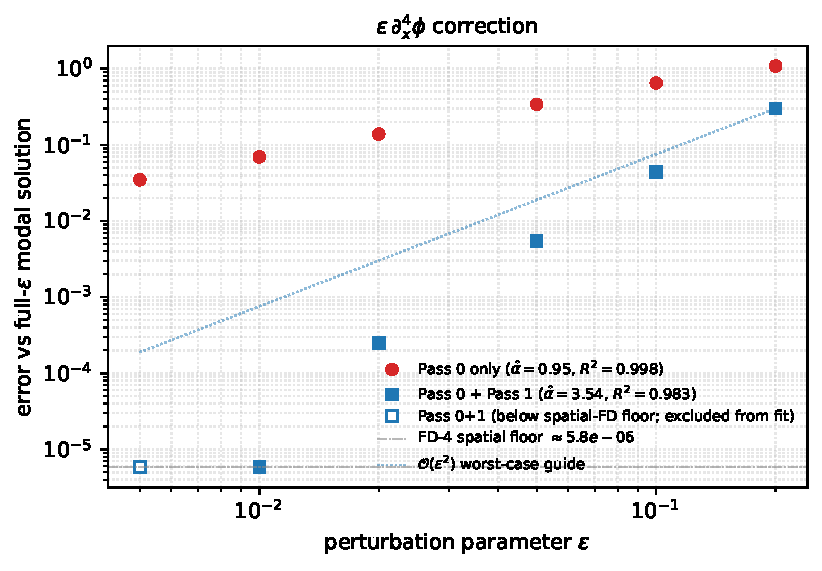
\includegraphics[width=\columnwidth]{figures/figD_parker_simon}
  \caption{Higher-derivative perturbative calibration. Pass 0 and
    Pass 0 + Pass 1 error versus $\varepsilon$ for the biharmonic
    correction \cref{KGBiharmonic} on the Klein--Gordon base of
    \cref{KGMassShift}. The combined-path error falls faster than
    the worst-case $\mathcal{O}(\varepsilon^2)$ bound at small
    $\varepsilon$. Points below the FD-4 spatial-discretisation
    floor (annotated in the figure) are excluded from the slope
    fit and shown as open markers.}
  \label{ParkerSimon}
\end{figure}

\paragraph*{Convention-anchored agreement with Euler--Heisenberg QED birefringence}
The QED Euler--Heisenberg effective action in the weak-field
limit~\cite{heisenberg1936consequences,schwinger1951gauge,dunne2004heisenberg}
is, to leading order in the field strength,
\begin{equation}
  \lag_{\mathrm{EH}} \;=\;
    \frac{2\alpha^{2}}{45\,m_{e}^{4}}\left[
      \bigl(\FieldF{_{\mu\nu}}\FieldF{^{\mu\nu}}\bigr)^{2}
      + \tfrac{7}{4}\bigl(\FieldF{_{\mu\nu}}\FieldFtilde{^{\mu\nu}}\bigr)^{2}
    \right],
  \label{LagEH}
\end{equation}
with $\alpha$ the fine-structure constant and $m_{e}$ the electron
mass. This gives a vacuum birefringence with refractive-index shifts
$n_\perp - 1 = (8\alpha^2/45)(B/B_c)^2$ and
$n_\parallel - 1 = (14\alpha^2/45)(B/B_c)^2$~\cite{adler1971photon},
giving the canonical ratio~\cite{dunne2004heisenberg}
\begin{equation}
  \frac{n_\parallel - 1}{n_\perp - 1} \;=\; \frac{7}{4}.
  \label{EHRatio}
\end{equation}
\TIDAL{}'s symbolic stage produces both absolute coefficients
analytically at the convention mapping $\sigma/\rho = 7/16$, in full
accordance with~\cite{adler1971photon}; the agreement is at the level
of individual coefficients rather than the ratio alone. An
independent measurement-path cross-check derives
$H_1/H_0 = -3\,(n_\perp - 1)_\mathrm{Adler}$ from the symbolic
Hamiltonian on the order-$\varepsilon^{0}$ trajectory, with no
involvement of the equation-of-motion solver.

\paragraph*{Cross-formulation equivalence: fundamental-vector versus
TorsionCDT}\label{FVCDTEquivalence}
For complex PGT theories where no closed-form solution and no
weak-field analytic limit is available --- the bulk of the
\cref{SectorSurvey} campaigns --- the only available consistency
check is to derive the same continuum action through two
mathematically distinct field formulations and verify that the
observables agree at the IEEE round-off limit. The
dark-photon-plasma sector affords this comparison directly. The
\emph{fundamental-vector} (FV) representation expresses the
torsion-coupling as a Proca-like massive vector field
$t_\mu$~\cite{caputo2021darkphoton},
\begin{equation}
  \mathcal{L}_\mathrm{FV} \;\supset\;
   -\tfrac14 \xi\,(\partial T)^2
   - \tfrac12 m_T^2\,t\!\cdot\! t
   + \delta_m\,F\!\cdot\!(\partial T),
  \label{LagFV}
\end{equation}
carrying $10$ dynamical fields with a clean kinetic structure
($\operatorname{cond}(V) \sim 10^{8\text{--}10}$); the
\emph{TorsionCDT} representation uses the irreducible-torsion
decomposition of~\cite{hehl1995metric,itin2004maxwell} with a
constrained-dyad kinetic ansatz (parameterised by the kinetic
prefactor $\xi$, the gauge-coupling shift $\alpha_3$, and the mass
mixing $\delta_m$; the Lagrangian appears with the dark-photon-plasma
sector in \cref{SectorSurvey}), carrying $18$ fields including
redundant constrained directions
($\operatorname{cond}(V) \sim 10^{15\text{--}17}$). The continuum
equivalence is recovered under the map $m_T^2 = +2\alpha_3$, derived
by squaring the FV mass term and identifying it with the trace
contribution to $I_3$. Across five canonical parameter points
spanning the surveyed sector the two formulations agree on $\Pmax$
to a relative difference at the IEEE-754 round-off floor of
$2.22\times 10^{-16}$, preserved at the same level across all
points.

Four implementation choices are validated against this
cross-formulation comparison:
\begin{itemize}
  \item Off-grid plane-wave initial conditions on a periodic grid
    leak amplitude onto every discrete Fourier mode
    (\cref{ICPreparation}); the solver snaps the requested
    initial-condition wavevector to the nearest discrete Fourier
    mode, and agreement holds with the snap but fails without it.
  \item For the TorsionCDT representation the eigenvector matrix
    becomes ill-conditioned above the double-precision threshold
    $\operatorname{cond}(V) \gtrsim 10^{13}$
    flagged by~\cite{higham2008functions}; the base evolution uses
    the scaling-and-squaring matrix exponential
    of~\cite{higham2009scaling} and the order-$\varepsilon^{1}$
    correction uses the augmented matrix exponential
    of~\cite{almohy2011action}, neither of which forms $V^{-1}$.
  \item The generalised-eigenvalue path is preceded by an SVD
    null-space projection to remove spurious finite eigenvalues on
    the rank-deficient TorsionCDT kinetic matrix.
  \item A modal-operator template cache is not used: a candidate
    implementation drifted by $0.36\%$ under parameter changes in
    inference posteriors, in violation of the linearity it assumed.
\end{itemize}
\Cref{FVCDT} displays the per-point relative difference. The
equivalence is a cross-formulation consistency check rather than an
independent reproduction of an analytic limit; it is the diagnostic
available on the linearisation, constraint-elimination, and
numerical-evolution paths for the complex PGT theories surveyed in
\cref{SectorSurvey}.

\begin{figure*}[t]
  \centering
  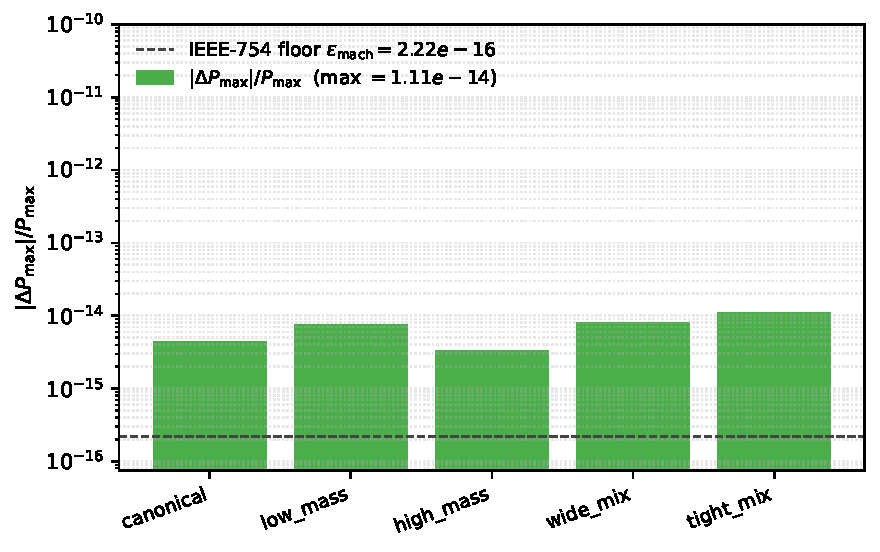
\includegraphics[width=\textwidth]{figures/figD_fv_cdt}
  \caption{Cross-formulation equivalence between the
    fundamental-vector representation \cref{LagFV} and the
    TorsionCDT representation (\cref{SectorSurvey}) of the
    dark-photon-plasma sector. Relative difference
    $|\Delta\Pmax|/\Pmax$ across the five canonical parameter
    points on a logarithmic axis, with the IEEE-754 round-off floor
    drawn for reference; the criterion is that all bars sit at or
    just above the floor.}
  \label{FVCDT}
\end{figure*}

\paragraph*{Multi-method agreement across backends and measurement paths}
\TIDAL{} dispatches to one of several solver backends according to
the equation specification (see \cref{SolverDispatchFlowchart}); we
calibrate the dispatcher by running representative theories under
every applicable backend and checking pairwise relative agreement
in $\Pmax$. Six backends --- modal, \CVODE{}, \IDA{}, leapfrog
Yoshida-2, leapfrog Yoshida-4, and \SciPy{}
DOP853~\cite{hindmarsh2005sundials} --- are exercised on the
Einstein--Maxwell baseline of \cref{GertsenshteinFormula} and on a
gradient-coupled scalar pair that is the analogue of the
Raffelt--Stodolsky two-channel mixing
model~\cite{raffelt1988mixing}. \SciPy{} Radau and BDF are excluded
on this benchmark: their implicit BDF/Radau Newton iteration
fails to converge on wave problems at the surveyed grid sizes; the
implicit family is already represented by \CVODE{} and \IDA{}. The
same calibration also runs a measurement-path cross-check: $H(t)$
derived from the symbolic Hamiltonian (Parseval gradient energy on
periodic domains) is compared to the EOM-based energy diagnostic,
two independent code paths for the same physical quantity. The
modal and \CVODE{} backends agree at the precision floor of the
modal evolution; explicit leapfrog and implicit \IDA{} agree with
the modal--\CVODE{} pair within their default integration
tolerances. \Cref{MultiMethod} displays the backend-pair heatmap on
each theory. These are internal-consistency checks across
independent computational paths; only the calibrations against
external analytic predictions in the earlier paragraphs constitute
independent reproductions.

\begin{figure*}[t]
  \centering
  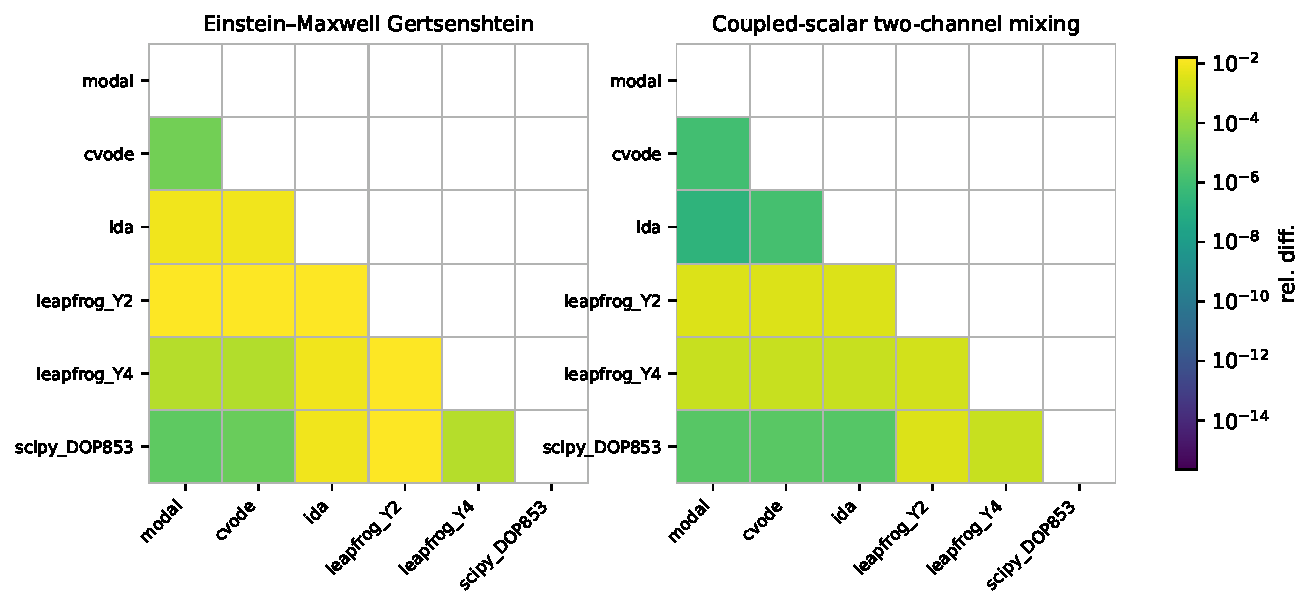
\includegraphics[width=\textwidth]{figures/figD_multi_method}
  \caption{Multi-method agreement across solver backends. Pairwise
    $\Pmax$ relative-difference heatmaps on the Einstein--Maxwell
    Gertsenshtein baseline (left) and the gradient-coupled scalar
    pair (right), the latter an analogue of the Raffelt--Stodolsky
    two-channel mixing model~\cite{raffelt1988mixing}. Logarithmic
    viridis colormap; cells encode
    $|P_a - P_b|/\max(|P_a|, |P_b|)$ between backend pairs $(a, b)$.
    Per-theory min, median, and max rel\_diff are annotated below
    each panel.}
  \label{MultiMethod}
\end{figure*}

\paragraph*{Spatial and temporal convergence}\label{ConvergenceCalibration}
The spatial-operator catalogue is calibrated against analytic
derivatives in \cref{FDConvergence}, where the Fornberg
finite-difference orders 2, 4 and 6 recover their predicted
algebraic rates and the pseudo-spectral path falls to the round-off
floor by $N\approx 64$~\cite{fornberg1988generation,burns2020dedalus}.
We extend the spatial calibration to a physical example by running
the Proca-mass equation at $\Bzero=0$ for a $k$-sweep at three
values of $m^2 \in \{0.1, 1.0, 10.0\}$; for each $(k, m^2)$ the
angular frequency is recovered by spatial-FFT identification of the
dominant mode, time-FFT of its complex amplitude with a Hann window,
and quadratic peak refinement, then compared to
$\omega(k) = \sqrt{k^2 + m^2}$. The Rabi-frequency grid convergence
runs on the Einstein--Maxwell baseline with the Rabi period chosen
to fit several full cycles inside the simulation window, and exposes
the $(k\Delta x)^2$ scaling of the fourth-order FD stencil error as
$N$ varies~\cite{fornberg1988generation}. Time-integration convergence
is reported only for the symplectic family (leapfrog Yoshida-2 and
Yoshida-4)~\cite{yoshida1990symplectic,hairer2006geometric}, where
the log--log slope of the absolute error versus $\Delta t$ is a
meaningful order-of-convergence diagnostic; implicit schemes
saturate at their rtol setting and their behaviour is covered in
\cref{MultiMethod}. \Cref{ConvergenceFigure} displays the three
diagnostics with fitted slopes and $R^2$ values annotated in each
legend. These calibrate discretisation and integrator order against
analytic targets; they do not probe modelling errors upstream of
the discretised system.

\begin{figure*}[t]
  \centering
  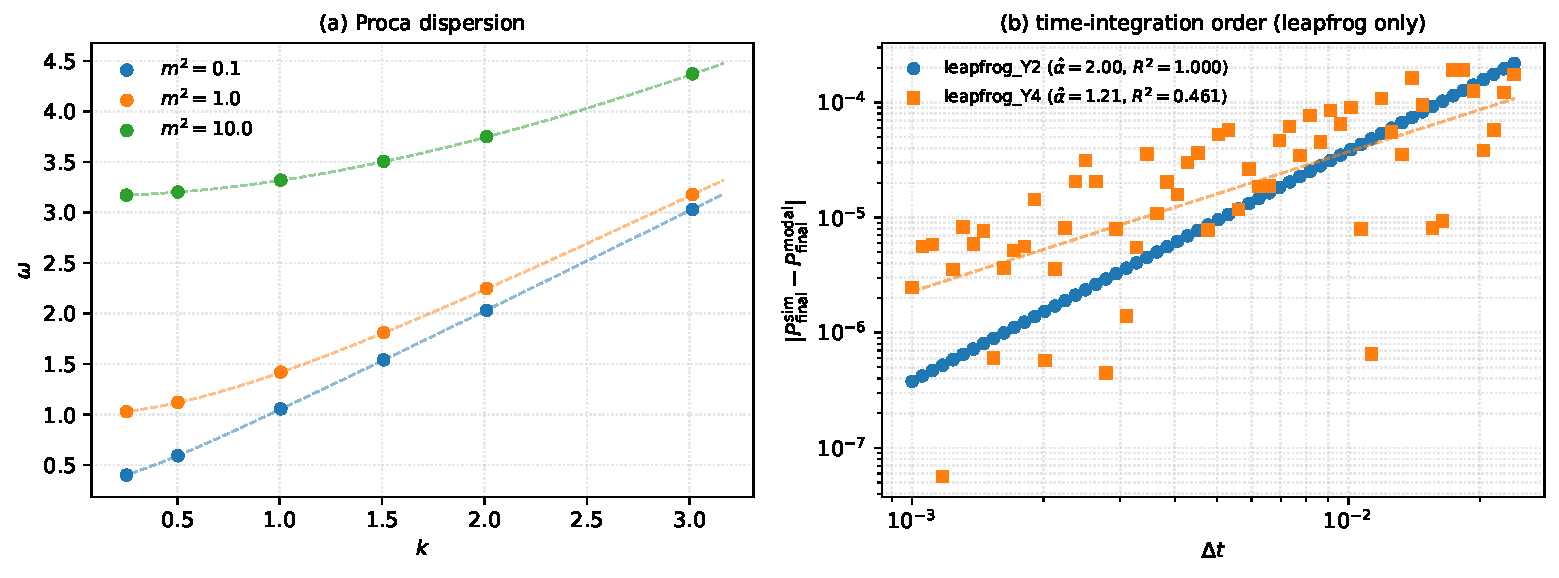
\includegraphics[width=\textwidth]{figures/figD_convergence}
  \caption{Spatial and temporal convergence. (a) Proca dispersion
    $\omega(k)$ extracted by FFT from \TIDAL{} at $m^2 \in \{0.1, 1, 10\}$,
    overlaid with the analytic $\omega = \sqrt{k^2 + m^2}$.
    (b) Rabi-frequency grid convergence
    $|\Omega_\mathrm{eff}/\Omega_\mathrm{theory} - 1|$ as a function
    of $k\Delta x$, at $\Bzero = 0.2$ and $t_\mathrm{end} = 200$
    (capturing $\approx 6.4$ Rabi periods); the residual is set by
    the FFT-extraction bin width rather than the spatial stencil
    over the surveyed $N$ range, and the plateau value is annotated
    on the figure. (c) Time-integration error versus $\Delta t$ for
    leapfrog Yoshida-2 and Yoshida-4 on the Einstein--Maxwell
    baseline; fitted log--log slopes and $R^2$ values are reported
    in the legend.}
  \label{ConvergenceFigure}
\end{figure*}

\paragraph*{Energy-conservation audit across the example library}
Energy conservation provides a structural diagnostic that engages
every layer of the workflow at once: a constraint solver that
returns inconsistent initial conditions, a symbolic stage that
loses cross-coupling terms in field decomposition, or a time
integrator that drifts past its predicted order, all surface as
relative energy drift. We audit the canonical example library and
record the maximum relative energy drift $|dE/E|_\mathrm{max}$ per
example: the Einstein--Maxwell Gertsenshtein baseline, the
gradient-coupled scalar pair, the propagating-PGT and nonminimal
torsion variants of \cref{SectorSurvey}, the dark-photon-plasma
sector in both fundamental-vector and TorsionCDT formulations, the
Proca-mass photon, and several flat- and curved-background
Klein--Gordon tests. Successful examples cluster at $\sim
10^{-15}$, near the IEEE-754 round-off floor of the modal solver.
Two structurally distinct outliers are documented separately and
not included in the calibration figure: the de-Sitter Klein--Gordon
example, where the energy drift is the physical Hubble friction of
the expanding background; and the massive rank-three antisymmetric
tensor example, whose Hamiltonian is omitted from the symbolic
stage because the Lagrangian decomposition cost is super-exponential
in tensor rank and exceeds the available compute budget. The audit
catches structural regressions, not per-example precision: the
precision floor is set by the backend the dispatcher selects, which
differs across examples. \Cref{ConservationAudit} displays the
per-example drift on a logarithmic axis, sorted in descending order.

\begin{figure}[t]
  \centering
  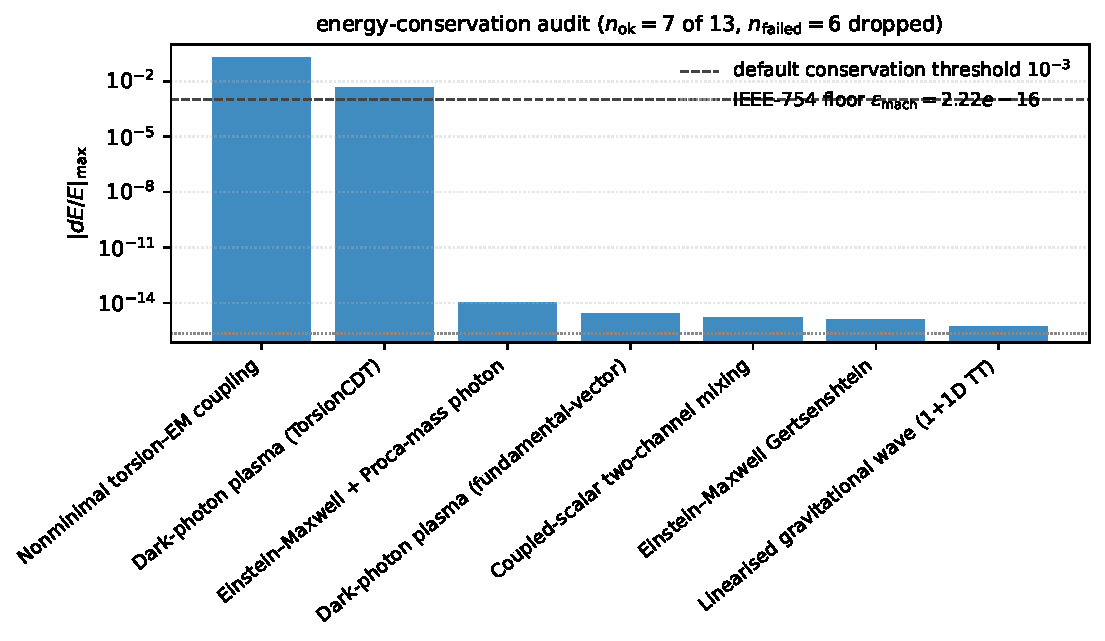
\includegraphics[width=\columnwidth]{figures/figD_conservation}
  \caption{Energy-conservation audit across the example library.
    Maximum absolute relative energy drift $|dE/E|_\mathrm{max}$ per
    example on a logarithmic axis, sorted in descending order. The
    default $10^{-3}$ conservation threshold (dashed) and the
    IEEE-754 round-off floor (dotted) are drawn for reference.
    Structurally distinct outliers (de-Sitter Klein--Gordon under
    physical Hubble friction; massive rank-three antisymmetric
    tensor with no symbolic Hamiltonian) are dropped from the
    audit and discussed separately in the text.}
  \label{ConservationAudit}
\end{figure}

\paragraph*{Torsion-limit recovery as a kinematic identity}
The propagating-PGT theory of \cref{PropagatingKineticOutput}
reduces to the Einstein--Maxwell baseline bit-exactly in the
$h_\times \leftrightarrow a_x$ channel across the surveyed $\xi$
range (which approaches $\xi = 0$ from above; the point $\xi = 0$
itself is degenerate as the torsion kinetic term vanishes there).
The agreement follows from the kinematic identity reported in
\cref{ChannelStructure}: the $h_\times \leftrightarrow a_x$ block
of the kinetic and coupling matrices does not depend on $\xi$ in
any sampled configuration, so the bit-equal agreement at every
sampled $\xi$ is structural rather than a calibration against an
analytic limit.

% Detail figures for §4.2 / §4.3 (status:stub in publication manifest,
% pending sector campaigns). Captions remain procedural and will be
% tightened during the §4 sector-survey drafting session.
\begin{figure}[t]
  \centering
  %TODO \includegraphics[width=\linewidth]{figures/figD1_stageA_heatmap}
  \caption{Stage A parameter-plane heatmap supporting the
    \cref{SectorSurveyTable} row for the dark-photon-plasma sector.}
  \label{StageAHeatmap}
\end{figure}

\begin{figure}[t]
  \centering
  %TODO \includegraphics[width=\linewidth]{figures/figD2_stageB_sweep}
  \caption{Stage B sweep scatter supporting the
    \cref{SectorSurveyTable} row for the torsion-coupling sector.}
  \label{StageBSweep}
\end{figure}

\begin{figure}[t]
  \centering
  %TODO \includegraphics[width=\linewidth]{figures/figD3_channel_comparison}
  \caption{Channel comparison supporting \cref{ChannelStructure}:
    $h_\times \leftrightarrow a_x$ time evolution vs the trace
    channel at the same $\Bzero$.}
  \label{ChannelComparison}
\end{figure}
